\documentclass[a4paper,10pt,onecolumn]{article}

\usepackage[T1]{fontenc}
\usepackage[utf8]{inputenc}
\usepackage{geometry}
% \geometry{a4paper,margin=10mm}
\usepackage[english]{babel}
\usepackage{natbib}
% \setcitestyle{authoryear,open={((},close={))}}

\usepackage{amsmath}
\usepackage{amssymb}

\usepackage{xcolor}
\usepackage{graphicx, url}
\usepackage{grffile}

\graphicspath{{../assets/}}

\usepackage{subcaption}

\usepackage{booktabs}

\title{Bayesian Sparsification of Deep $\cplx$-valued networks}
\author{Ivan Nazarov, and Evgeny Burnaev}

%% notation
\newcommand{\real}{\mathbb{R}}
\newcommand{\cplx}{\mathbb{C}}

\begin{document}
\maketitle
\listoffigures

\clearpage

\begin{figure}[b]
  \centering
  \begin{subfigure}[b]{0.5\columnwidth}
    \centering
    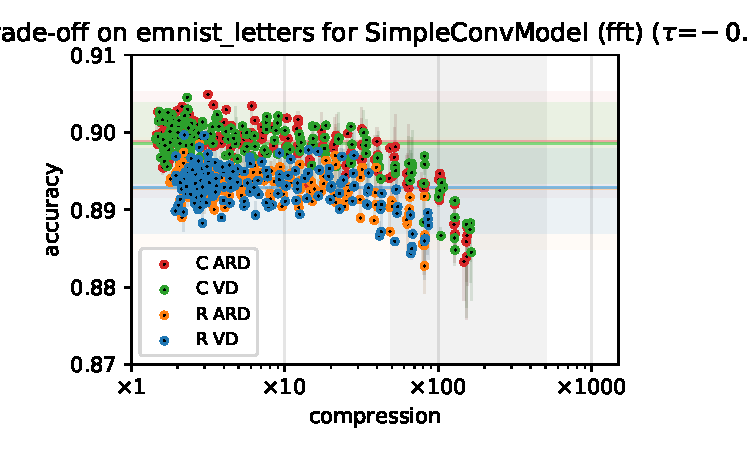
\includegraphics[width=\columnwidth]{figure__mnist-like__method_comparison/appendix__SimpleConvModel__emnist_letters__fft__-0.5.pdf}
  \end{subfigure}%
  \begin{subfigure}[b]{0.5\columnwidth}
    \centering
    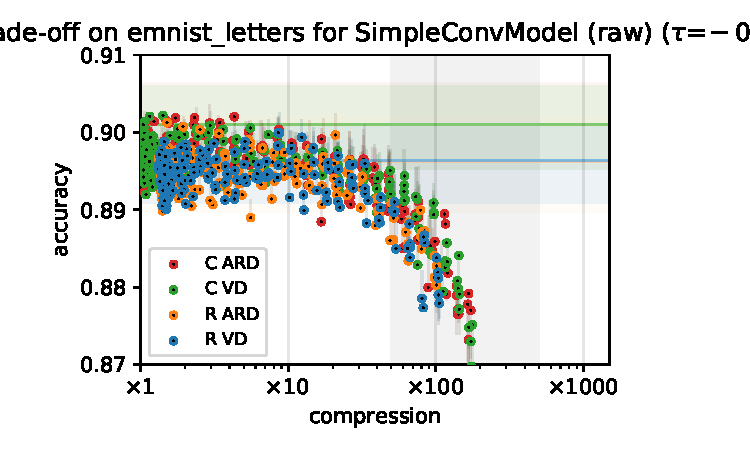
\includegraphics[width=\columnwidth]{figure__mnist-like__method_comparison/appendix__SimpleConvModel__emnist_letters__raw__-0.5.pdf}
  \end{subfigure} \\ %
  \begin{subfigure}[b]{0.5\columnwidth}
    \centering
    % used in main text
    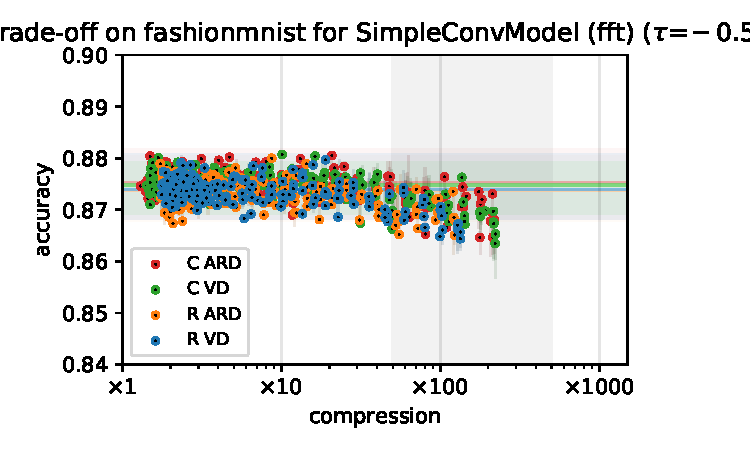
\includegraphics[width=\columnwidth]{figure__mnist-like__method_comparison/appendix__SimpleConvModel__fashionmnist__fft__-0.5.pdf}
  \end{subfigure}%
  \begin{subfigure}[b]{0.5\columnwidth}
    \centering
    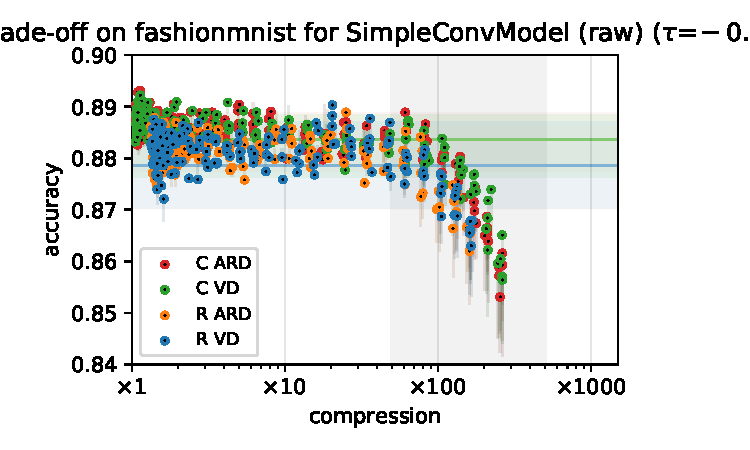
\includegraphics[width=\columnwidth]{figure__mnist-like__method_comparison/appendix__SimpleConvModel__fashionmnist__raw__-0.5.pdf}
  \end{subfigure} \\ %
  \begin{subfigure}[b]{0.5\columnwidth}
    \centering
    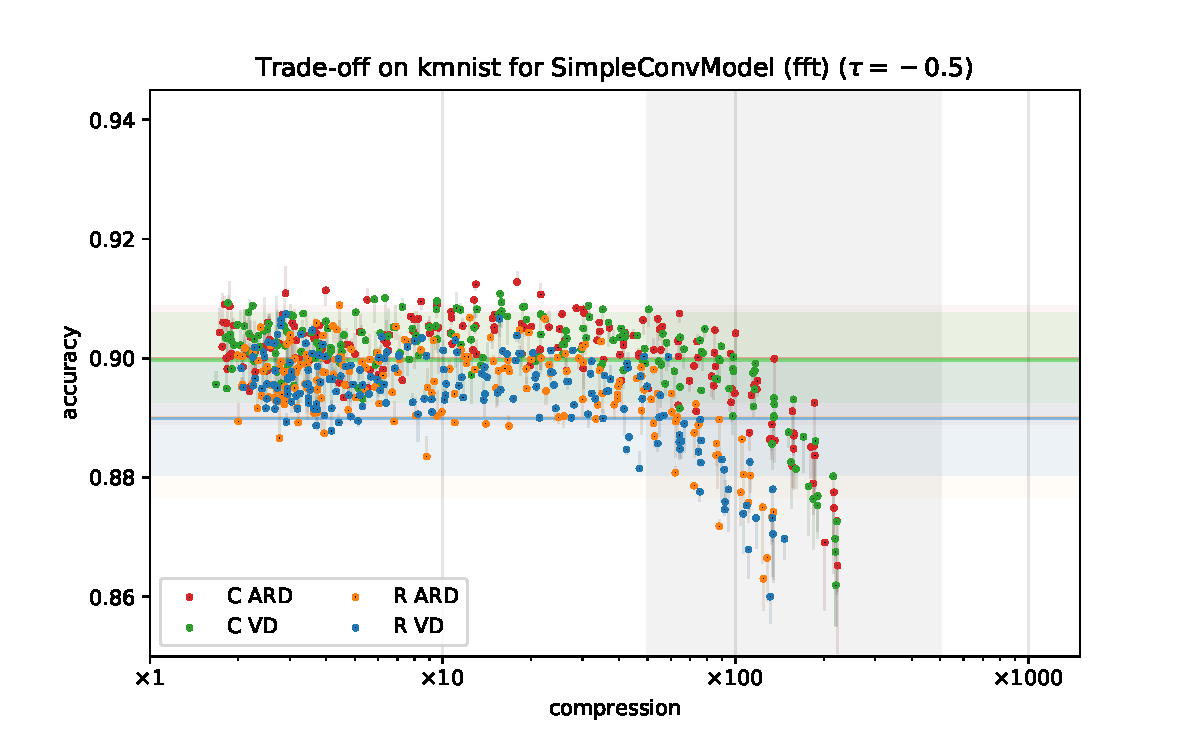
\includegraphics[width=\columnwidth]{figure__mnist-like__method_comparison/appendix__SimpleConvModel__kmnist__fft__-0.5.pdf}
  \end{subfigure}%
  \begin{subfigure}[b]{0.5\columnwidth}
    \centering
    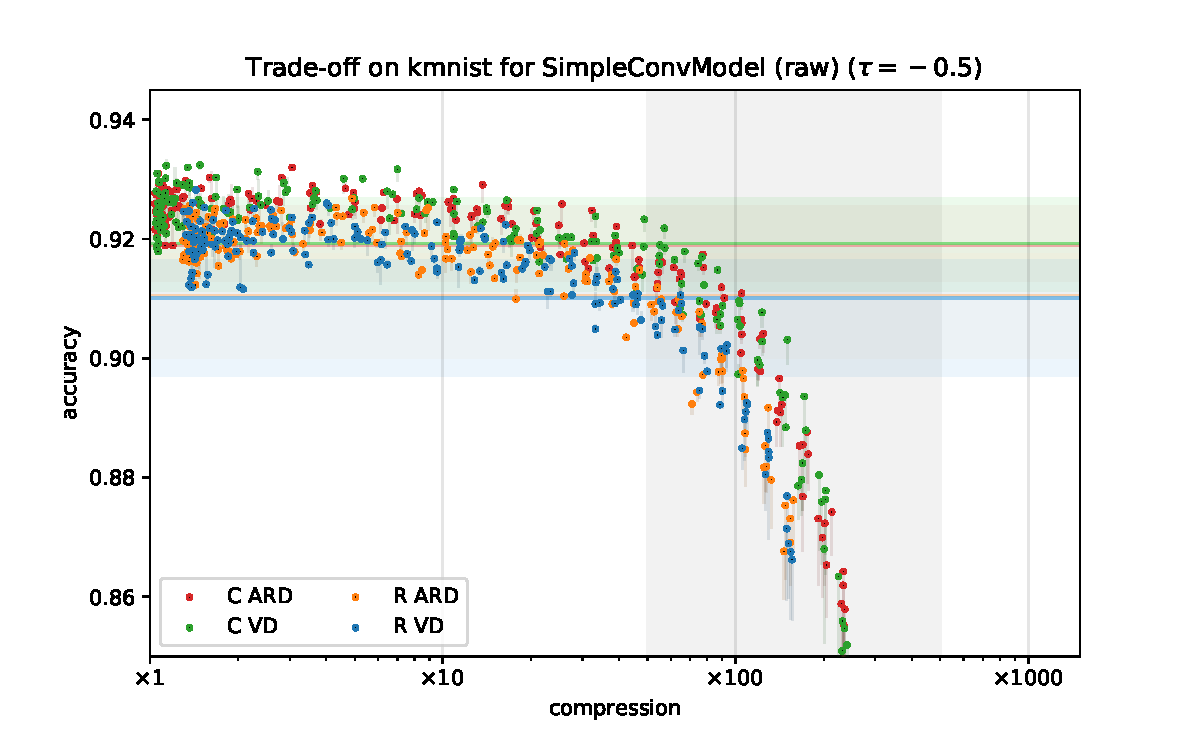
\includegraphics[width=\columnwidth]{figure__mnist-like__method_comparison/appendix__SimpleConvModel__kmnist__raw__-0.5.pdf}
  \end{subfigure} \\ %
  \begin{subfigure}[b]{0.5\columnwidth}
    \centering
    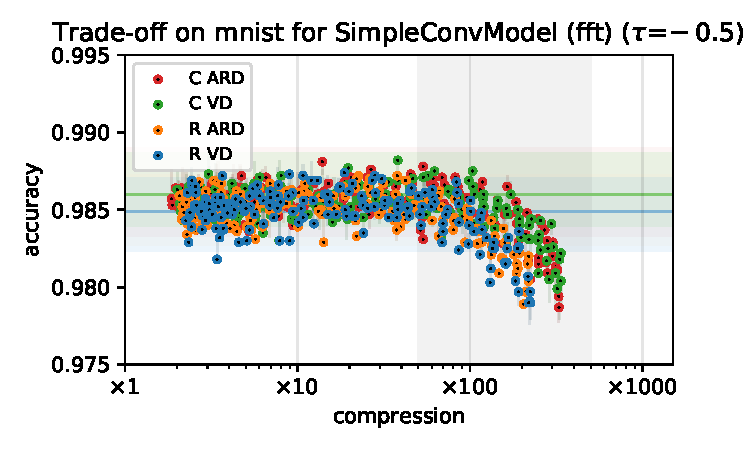
\includegraphics[width=\columnwidth]{figure__mnist-like__method_comparison/appendix__SimpleConvModel__mnist__fft__-0.5.pdf}
  \end{subfigure}%
  \begin{subfigure}[b]{0.5\columnwidth}
    \centering
    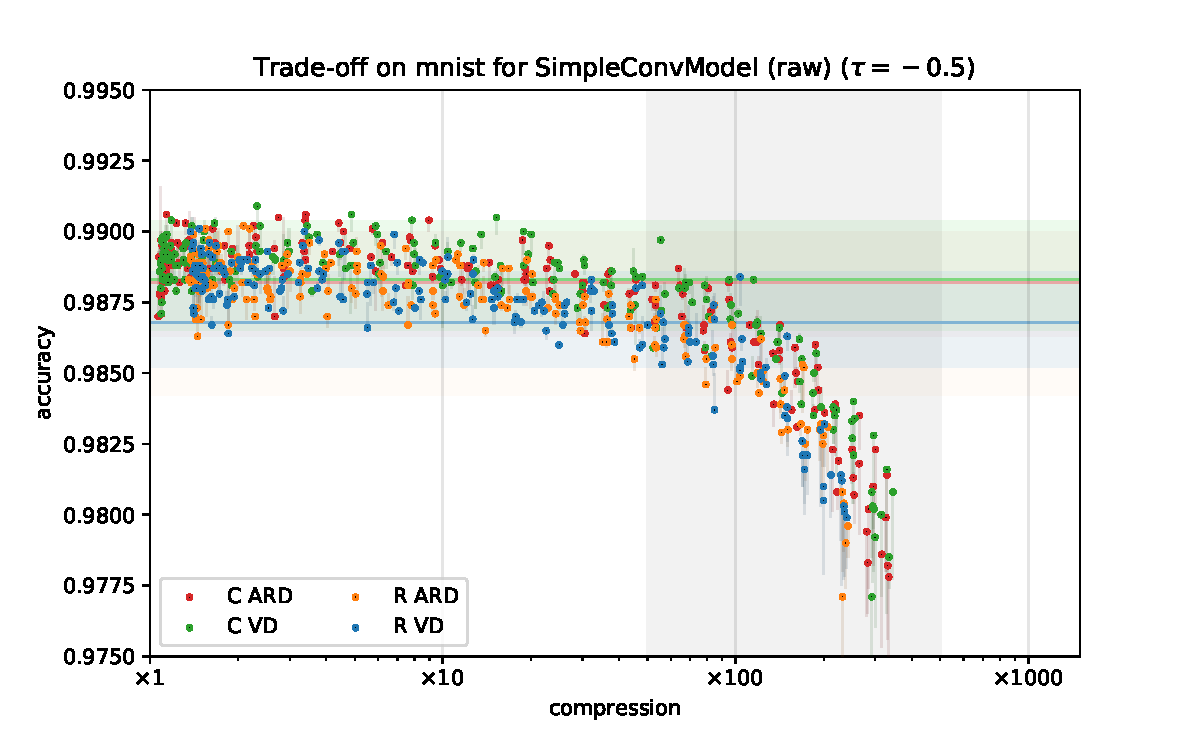
\includegraphics[width=\columnwidth]{figure__mnist-like__method_comparison/appendix__SimpleConvModel__mnist__raw__-0.5.pdf}
  \end{subfigure}
  \caption{%
    \texttt{SimpleConvModel}: (row 1) EMNIST, (rows 2) Fashion-MNIST, (row 3) KMNIST, (row 4) MNIST.
  }
  % \label{fig:appendix__mnist-like__trade-off__emnist_letters}
\end{figure}

\begin{figure}[b]
  \centering
  \begin{subfigure}[b]{0.5\columnwidth}
    \centering
    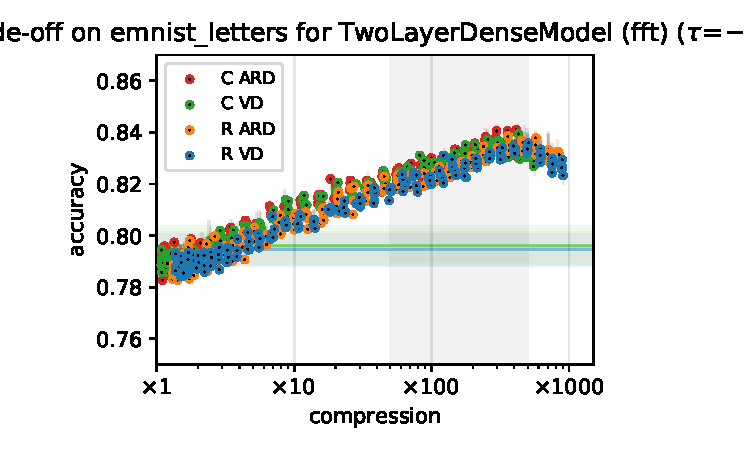
\includegraphics[width=\columnwidth]{figure__mnist-like__method_comparison/appendix__TwoLayerDenseModel__emnist_letters__fft__-0.5.pdf}
  \end{subfigure}%
  \begin{subfigure}[b]{0.5\columnwidth}
    \centering
    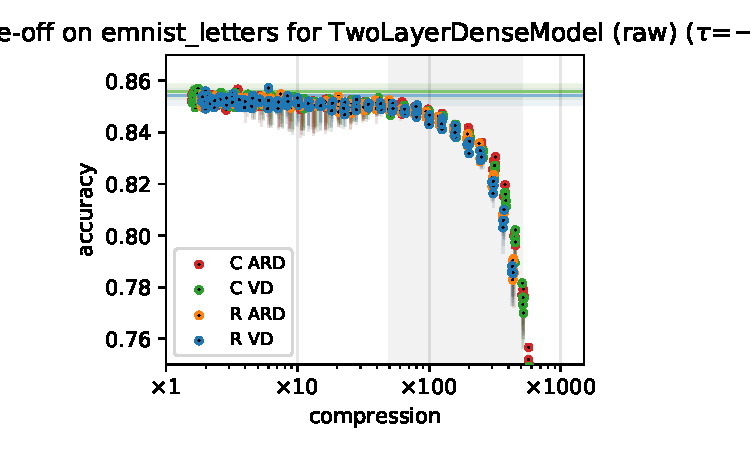
\includegraphics[width=\columnwidth]{figure__mnist-like__method_comparison/appendix__TwoLayerDenseModel__emnist_letters__raw__-0.5.pdf}
  \end{subfigure} \\ %
  \begin{subfigure}[b]{0.5\columnwidth}
    \centering
    % used in main text
    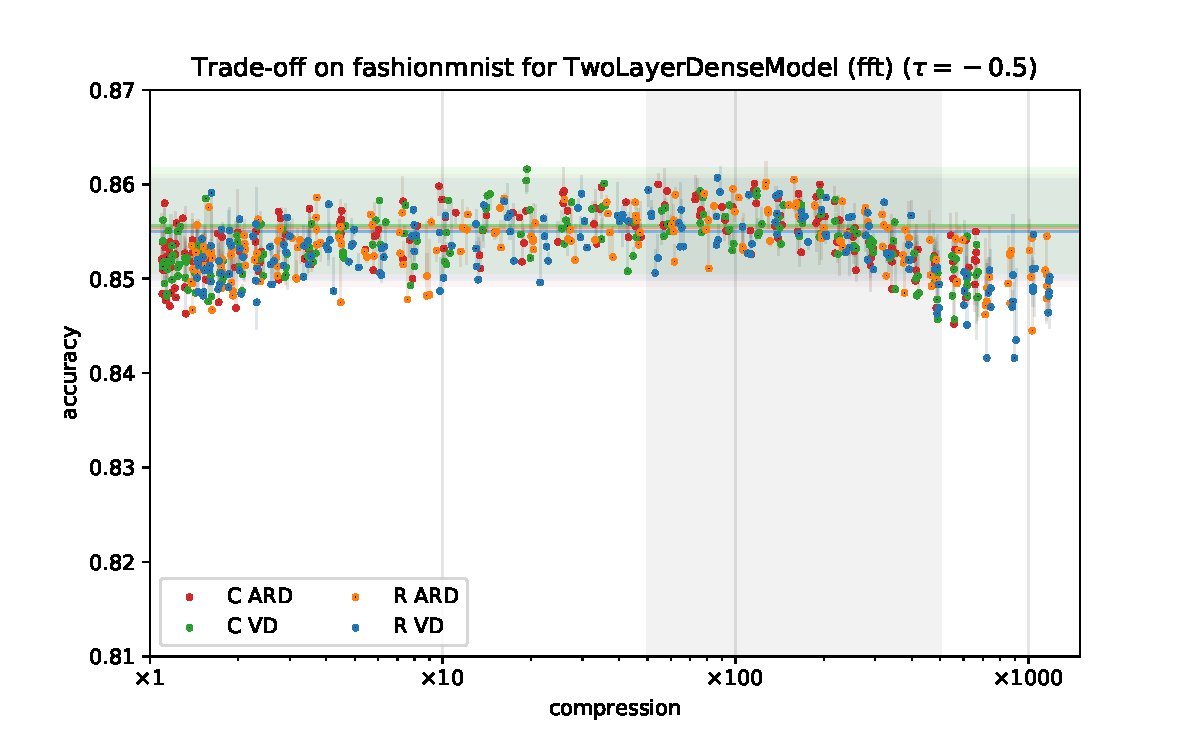
\includegraphics[width=\columnwidth]{figure__mnist-like__method_comparison/appendix__TwoLayerDenseModel__fashionmnist__fft__-0.5.pdf}
  \end{subfigure}%
  \begin{subfigure}[b]{0.5\columnwidth}
    \centering
    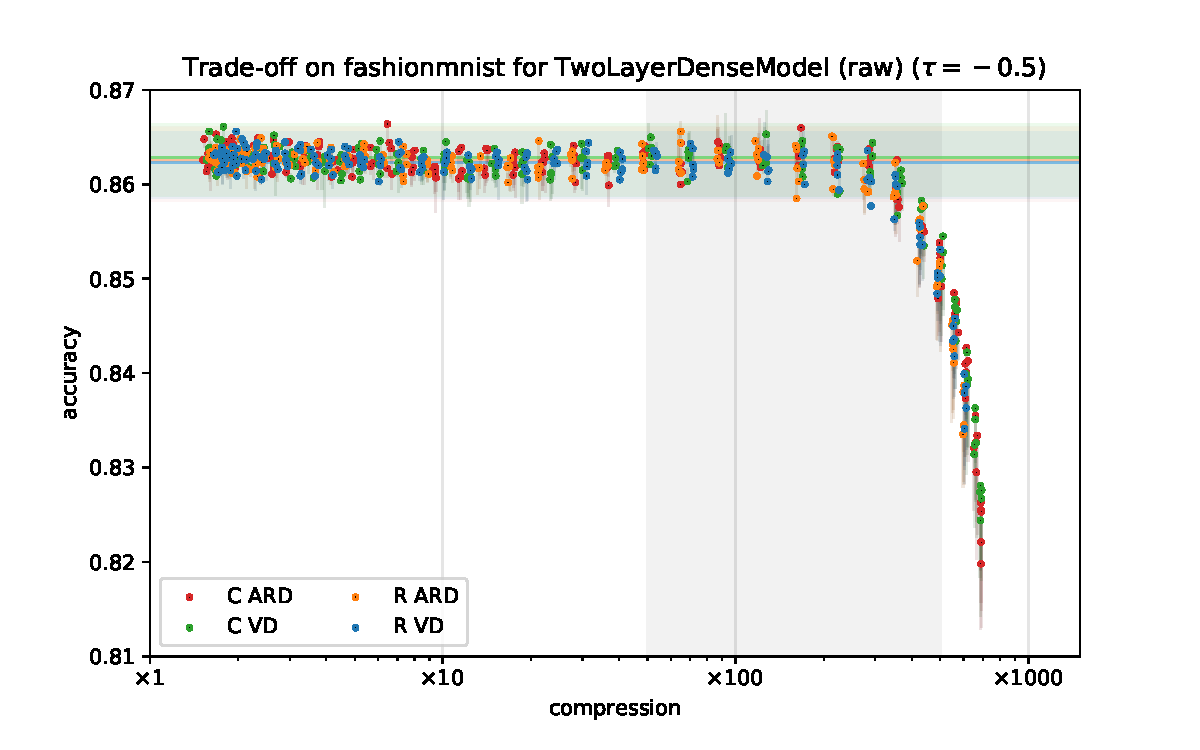
\includegraphics[width=\columnwidth]{figure__mnist-like__method_comparison/appendix__TwoLayerDenseModel__fashionmnist__raw__-0.5.pdf}
  \end{subfigure} \\ %
  \begin{subfigure}[b]{0.5\columnwidth}
    \centering
    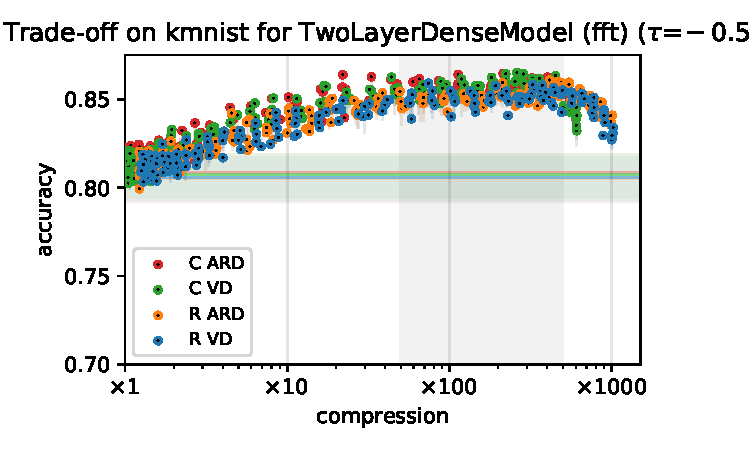
\includegraphics[width=\columnwidth]{figure__mnist-like__method_comparison/appendix__TwoLayerDenseModel__kmnist__fft__-0.5.pdf}
  \end{subfigure}%
  \begin{subfigure}[b]{0.5\columnwidth}
    \centering
    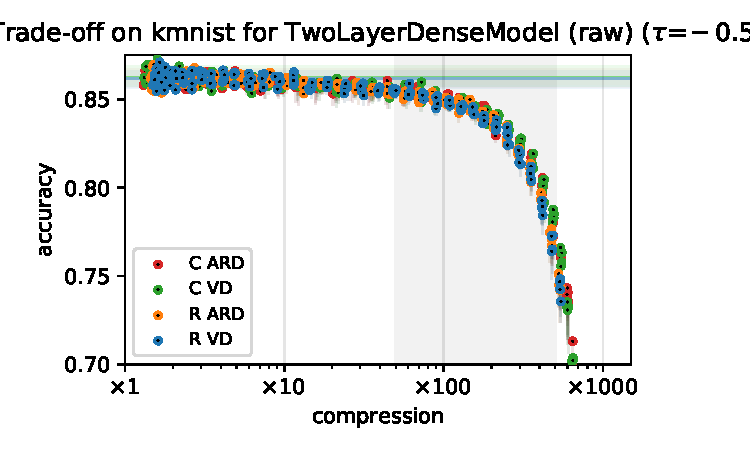
\includegraphics[width=\columnwidth]{figure__mnist-like__method_comparison/appendix__TwoLayerDenseModel__kmnist__raw__-0.5.pdf}
  \end{subfigure} \\ %
  \begin{subfigure}[b]{0.5\columnwidth}
    \centering
    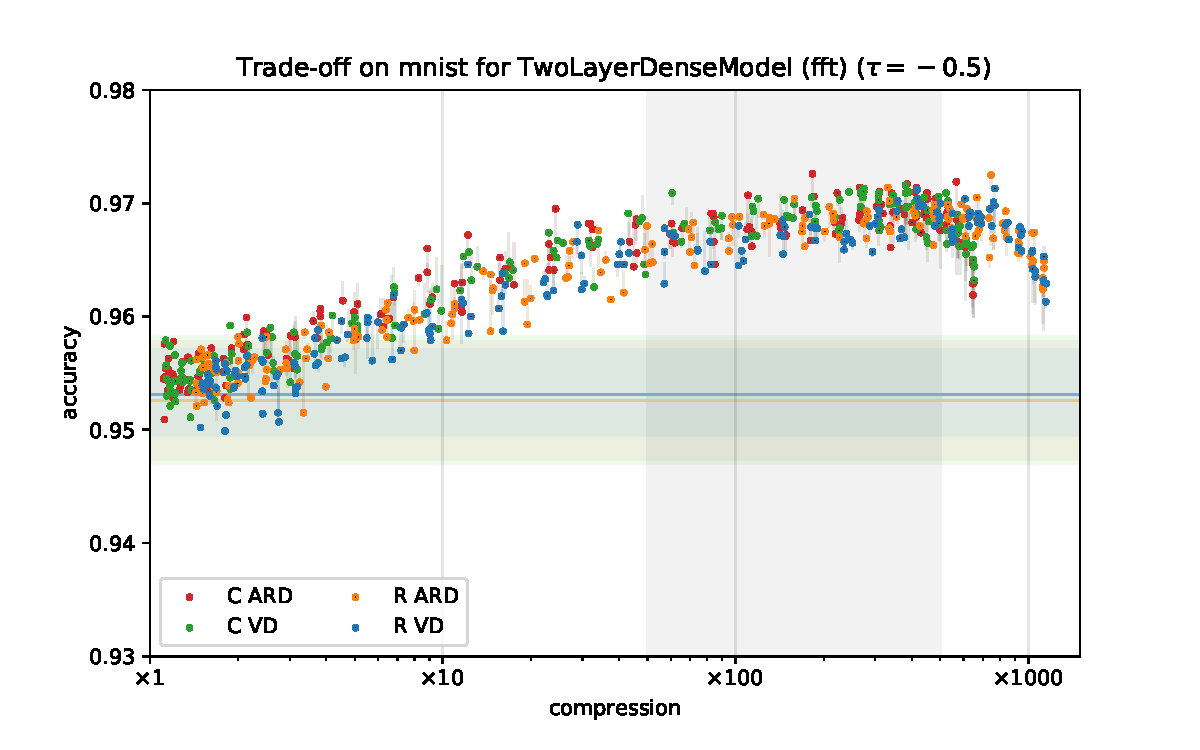
\includegraphics[width=\columnwidth]{figure__mnist-like__method_comparison/appendix__TwoLayerDenseModel__mnist__fft__-0.5.pdf}
  \end{subfigure}%
  \begin{subfigure}[b]{0.5\columnwidth}
    \centering
    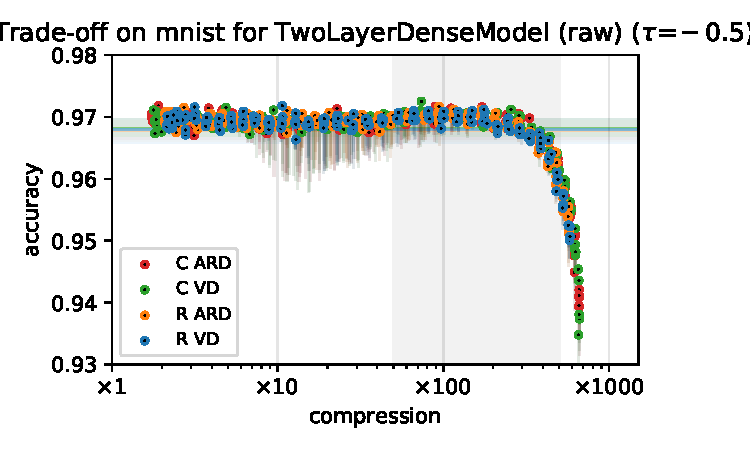
\includegraphics[width=\columnwidth]{figure__mnist-like__method_comparison/appendix__TwoLayerDenseModel__mnist__raw__-0.5.pdf}
  \end{subfigure}
  \caption{%
    \texttt{TwoLayerDenseModel}: (row 1) EMNIST, (rows 2) Fashion-MNIST, (row 3) KMNIST, (row 4) MNIST.
  }
  % \label{fig:appendix__mnist-like__trade-off__kmnist}
\end{figure}

\end{document}
